%----------------------------------------
% Preamble to set up the document
%----------------------------------------
\documentclass{article}

% set up packages (you shouldn't need to touch this)
\usepackage{graphicx}  % required to insert images
\usepackage{hyperref}  % for hyperlinks
\usepackage[svgnames]{xcolor}  % to change hyperlink colors
\colorlet{linkcolour}{DarkBlue}
\hypersetup{colorlinks=true, linkcolor=linkcolour, citecolor=linkcolour, urlcolor=linkcolour,}

% Margins
\topmargin=-0.45in
\evensidemargin=0in
\oddsidemargin=0in
\textwidth=6.5in
\textheight=9.0in
\headsep=0.25in

% use a sans serif font
\renewcommand{\familydefault}{\sfdefault}

%----------------------------------------
% Step 1: Edit the lecture title
%----------------------------------------
\title{
Lecture 4: Review of Data Operations, and Introduction to Data Visualization \\  % Lecture title
Modeling Social Data, Spring 2019 \\   % Course title
Columbia University                    % School
}

%----------------------------------------
% Step 2: Edit your name and the date
%----------------------------------------
\author{Ongun Uzay Macar}                     % Scribe's name
\date{February 15, 2019}                % Lecture date

\begin{document}

\maketitle


%----------------------------------------
% Step 3:
% Rename uni.tex to match your uni,
% edit the filename accordingly below,
% and put your notes in this file
%----------------------------------------
%----------------------------------------
% Write your notes here
%----------------------------------------

\section{Introduction}
This lecture, we reviewed basics and data operations in R, discussed why data visualization is important and how can we benefit from it, and lastly learned how to utilize the ggplot2, plotting library in R.

\section{Review of Basics and Data Operations}

In some cases, we may want to convert our data to a new format, and
this is often denoted as 'tidying data' . The R functions we will have
to know in particular for this purpose are 'gather()' and 'spread()'. 

\subsection{gather() and spread()}
\begin{itemize}
    \item Gather takes wide data and makes it long, by converting
    column names into actual values in the table. It is not guaranteed
    to be in order. 
    \item We have gone over the CitiBike example that is asked on the
    homework, where we convert start and stop time columns under a new
    variable column, and the respective times as Date objects under a
    value column. 
    \item We can then sort according to the dates and end up with a periodic time line.
    Hence, as start times and stop times are processed, we can keep a running count on
    active bikes and update accordingly to get the maximum number of active bikes on a
    given time. 
    \item With 'gather()' and piped operations, we can use the 'ifelse' block of base R
    which acts as a vectorized form of the conditional blocks seen in other languages. 
    \item One way is to use this block inside mutate() function to assign certain values
    to rows of your data.
    \item With 'spread()' on the other hand, we go from long to wide. This time, we take a
    row value and convert it to a column.
\end{itemize}
\subsection{Question: Are gather() and spread() inverses of each other?}
Although they are pretty close to being called 'inverses', formally \textbf{NO}, they are
not. This is because
\begin{enumerate}
    \item There is no guarantee in order, the data frame doesn't necessarily match going
    back and forth between these two operations. 
	\item There is no guarantee that all columns will contain values, there may be missing
	values.
\end{enumerate}

\subsection{Basics of R and RStudio}
\begin{itemize}
    \item In RStudio, we were introduced to the terminal, the environment which holds all
    your data and variables, the help section, and the file system. In overall, RStudio is
    a great development environment with many benefits.
    \item We saw how to load up a library with the simple library(libraryname)
    conventionally placed in the beginning of the file.
    \item We saw that we can use concatenation to easily create vectors in R. To create a
    vector over a range or interval, the seq() and c() functions come in handy.
    \item Vectors can have named columns. Hence, a value at an index may be accessed
    through vector[columnname]
    \item We can look at the structure of any object by calling str() function upon it. 
    \item If you cast a vector to a factor with the as.factor() function, the str()
    function will now give us the number of unique levels in the data. The plotting tools
    will know to treat these as categorical variables.
    \item We will not be using a lot of R 'lists'. Instead, data frames that hold tabular
    data are often much useful.
    \item \textbf{Quick R Tip}: If you are opening up a file and you are not finding
    something you are trying to load, it is probably because the working directory is not
    set to the source file location. You can do this from Session, Set Working Directory,
    To Source File Location.
\end{itemize}

\subsection{Data Operations}
\begin{itemize}
    \item The summary() function called upon a data frame will give minimum, maximum,
    median, mean, 1st Quartile, and 3rd Quartile values for numerical columns, and in the
    case of a factor column it gives a summary of the categorical levels. The adeptness of
    the summary() function comes in very handy while exploring and analyzing data.
    Below is only what is discussed in this class. Definitely go over this file (...) to
    learn about more nifty operations and functions in R.
    \item Old way is logical indexing to select rows through dollar sign column name and
    the logical operation inside the brackets, whereas the new way is to use the
    filter(logic) function. The new way is definitely more readable. The grepl() function
    returns a boolean value depending on whether the pattern is contained within the value
    or not. Used within filter(), it will act in vectorized form.
    \item In the new way, use arrange() to reorder rows, select() to select rows, mutate()
    to modify columns, and summarize() to summarize columns and extract information such
    as mean and standard deviation.
    \item To create a grouped data frame, use groupby() function which simulates the
    split/apply/combine procedure discussed in earlier lectures. Within this function,
    there are a bunch of helper methods that can be used like n() which gives you the
    number of rows, rownumber() which gives you 1,2,3,4,5,... (incremental indexing) for
    all the rows. 
    \item Ungrouping shouldn't be forgotten when you want to revert back to the original
    data frame format. Not remembering this step might cause us to get some unintended
    results and computations in our data analysis.
    \item Another reason to ungroup might be based on performance issues. When the data
    frame is grouped, any vectorized operation is going through each group and within each
    group, it is iterating which proves grouping to be a costly operation. 
    \item A filter() operation was demonstrated on a grouped data frame, where the
    operation is distributed to each group as result of the split/apply/combine process,
    and hence it takes a longer computational time than expected. The expected value in
    this case was the maximum value of the whole data frame, rather than the maximum value
    within each group as outputted. This often leads to confusion.
    \item The pipe operator, that is showcased with a data frame being chained into a
    series of vectorized operations, is a nice convention to use in R. It enhances
    readability, and decreases the complexity of the code.
\end{itemize}

\begin{figure}[ht]
  \begin{center}
    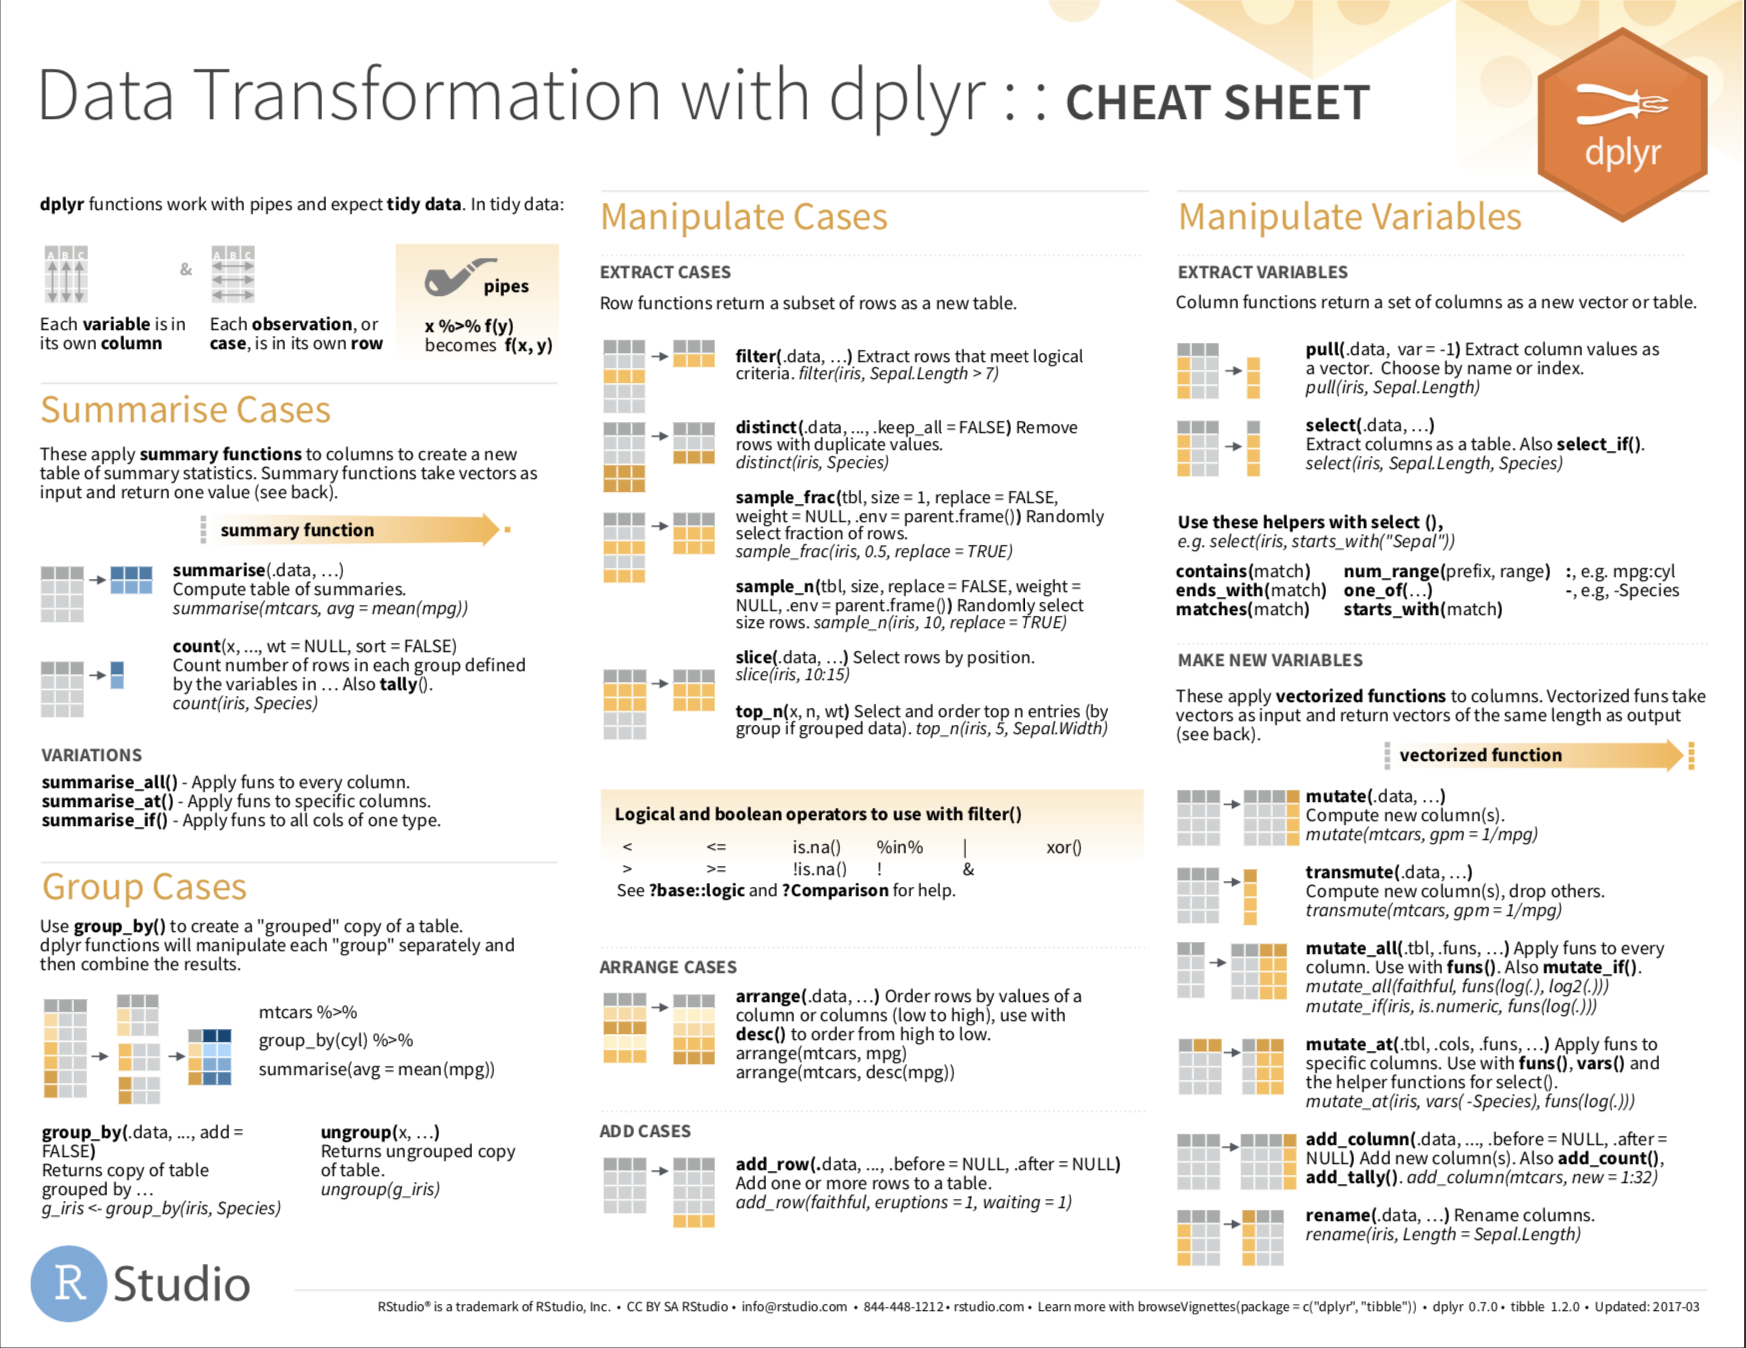
\includegraphics[width=1\textwidth]{figures/data_operations.png}
    \caption{Official RStudio Cheat Sheet for Data Transformation with 
    dplyr, https://www.rstudio.com/resources/cheatsheets/#dplyr}
    \label{fig:example_figure}
  \end{center}
\end{figure}

\section{Introduction to Data Visualization}
\subsection{Question: Why do you want to visualize data?}
\begin{itemize}
    \item To make full meaning and utility of data.
    \item Convey any results in an easily understandable fashion to the readers.
    \item The idea is to lower the cost of going from a idea on your mind to an actual, interpretive plot.
\end{itemize}
\subsection{Real Life Applications and Usage}
\begin{itemize}
    \item Professor Jake mentioned that often he has spent multiple hours on deciding
    figures and the types of plots he wanted to display. On projects he has worked,
    figures had often multiple revisions by many different people. All this is to say
    that, good data visualization takes a lot of practice and conveying information to
    readers through plots is an important tool.
    \item We have discussed about Anscombe's Quartet (1973) to understand why data
    visualization is important. The difference between the four data sets are really hard
    to tell just by looking at a data table. The spread, range, and the correlation
    between variables are especially hard to understand. When plotted, on the other hand,
    the difference is immediately a lot easier to interpret. 
    \item Now that we know about the existence of a powerful plotting library in R,
    ggplot2, we noted that we have so many options to choose from (histogram, density
    plot, cumulative density, boxplots, etc.) with regard to our display of the data. We
    even have many options about styling (shape, size, color, and line width properties of
    data). There are nice rules of thumb about how to do these things also things we can
    learn from practice.
    \item Good plots should accurately and effectively express the facts. Professor Jake
    has mentioned that he decides whether a plot is useful or not by attempting to
    construct a one sentence take-away or conclusion just by looking at the plot. Looking
    back to the slides from the first lecture, every figure and plot provided had a one
    sentence takeaway written beneath it.
    \item Cleveland and McGill (1984) experiments reveal that position and length are
    often more easily understood than color and density differences in plots.  Heer and
    Bostock (2010) has reproduced a similar ranking based of on data collected from
    Mechanical Turk. This is important, because it shows that visualization research can
    be done online instead of just depending of physical lab participants.
    \item In a seperate research by Jock Mackinlay, it has been shown that the ranking
    also depends on the type of data at hand. There are three possibilities:
    \begin{enumerate}
        \item Quantitative: numerical values in a range
        \item Ordinal: categories with natural ordering
        \item Nominal: categories with no natural ordering
    \end{enumerate}
    \item For example, using area to encode quantitative information makes more sense than
    with ordinal and nominal data. 
    \item We have seen that with annual median income (quantitative data), a plot on the
    map of the U.S. with different colors (darker blue indicates a higher income) was
    preferred. On the other hand, population growth (nominal data) was chosen to be
    represented reversed and sorted histogram where color now indicates the region of the
    state (West, South, Midwest, or Northeast).
\end{itemize}

\section{Data Visualization in R with ggplot2}
\subsection{Grammar of Graphics}
\begin{itemize}
    \item Grammar of graphics is the language to describe the components of a plot or a
    visual. This grammar usually follows a general guideline template with 5 steps:
\begin{enumerate}
    \item Get your data into the right format by tidying. 
    \item Map variables to aesthetics (color, shape, size)
    \item Choose a geometry for your plot. (different plot types)
    \item  Set co-ordinate system and scales (linear or log)
    \item Add annotations, legends, and labels. (x-axis, y-axis, title)
\end{enumerate}
    \item Then you get a plot at the end of the day. The aes() helper function takes care
    of the mappings for your plot inside the ggplot() function call.
\end{itemize}

\subsection{Benefits of ggplot2}
The benefits of ggplot2 comes directly with its conciseness and doing massive amounts of
work in less lines. Some other benefits mentioned are:
\begin{itemize}
    \item Lowers the barrier to asking questions of your data, lets you interpret easily
    using plots
    \item Lets you explore and analyze more, and faster
    \item Easily produces beautiful, publication-ready plots
    \item Large and activate user base for support
\end{itemize}

\subsection{Diving into ggplot2}
\begin{itemize}
    \item Usage is simple: ggplot(data, aes=(x = data, y = data)) where "aes" stands for
    aesthetic mapping.
    \item \textbf{Keep in mind}: The plus (+) sort of adds on stuff to the plot. It is not
    equivalent to pipe operator.
    \item geomhistogram() is the function to create a histogram. You should always set the
    bins of the histogram yourself through geomhistorgram(bins = number of bins)
    \item geompoint() gives a scatter plot. ggplot() takes care of spacing for you, which
    is very useful. 
    \item The piping operator is something we better get used to it because of it
    convenience. We can summarize the data and pipe the result immediately into ggplot. 
    \item geomline() creates line plots. Always include xlab(title) and ylab(title) to
    name your axes and enhance readibility. 
    \item geomline() + scaleylog10() gives a logged y-axis, which may make your data
    easier to understand from a plot. 
    \item To see an overall trend, we can use geomsmooth(method = "lm") to fit a linear
    model to the data and display it on top. We can combine geompoint() which will give
    regular points for actual data points, with geomsmooth(method = "lm") with the +
    operator which gives the best fit line for the model.
    \item We can filter out unwanted data points by
    \begin{enumerate}
        \item Simply excluding them from the visualization with coordcartesian(xlim =
        vector, ylim = vector). This will leave the best fit line and hence the
        representative model unchanged; only the display is changed.
        \item Use xlim(vector)or scalexcontinuous(lim = vector) to first filter the data,
        then change the fit accordingly, and finally display the new model.
        \item Extract the data yourself before plotting with data frame piped to
        filter(logic) function. This method may be used to prevent any kind of errors and
        confusions going forward.
    \end{enumerate}
    \item Pipe data frame to leftjoin(<dataframe>) function call to extend your data with
    more descriptive columns.
    \item Plotting a histogram of number of ratings by movie with the MovieLens data that
    is used in Homework 1, we observed that this data has a "long tailed" distribution.
    This means that whereas the bulk of the available movies draw little attention, a few
    movies get a lot of attention. 
    \item Use geomdensity(fill = color) to  have a smoothed version of the histogram. You
    can also include the mean in your plot as a dashed line with geomvline(aes(xintercept
    = mean(numratings)), linetype = "dashed")
    \item Use the cumsum(<data>)  function combined with ggplot() to get a cumulative
    distribution (CDF).
\end{itemize}

\begin{figure}[ht]
  \begin{center}
    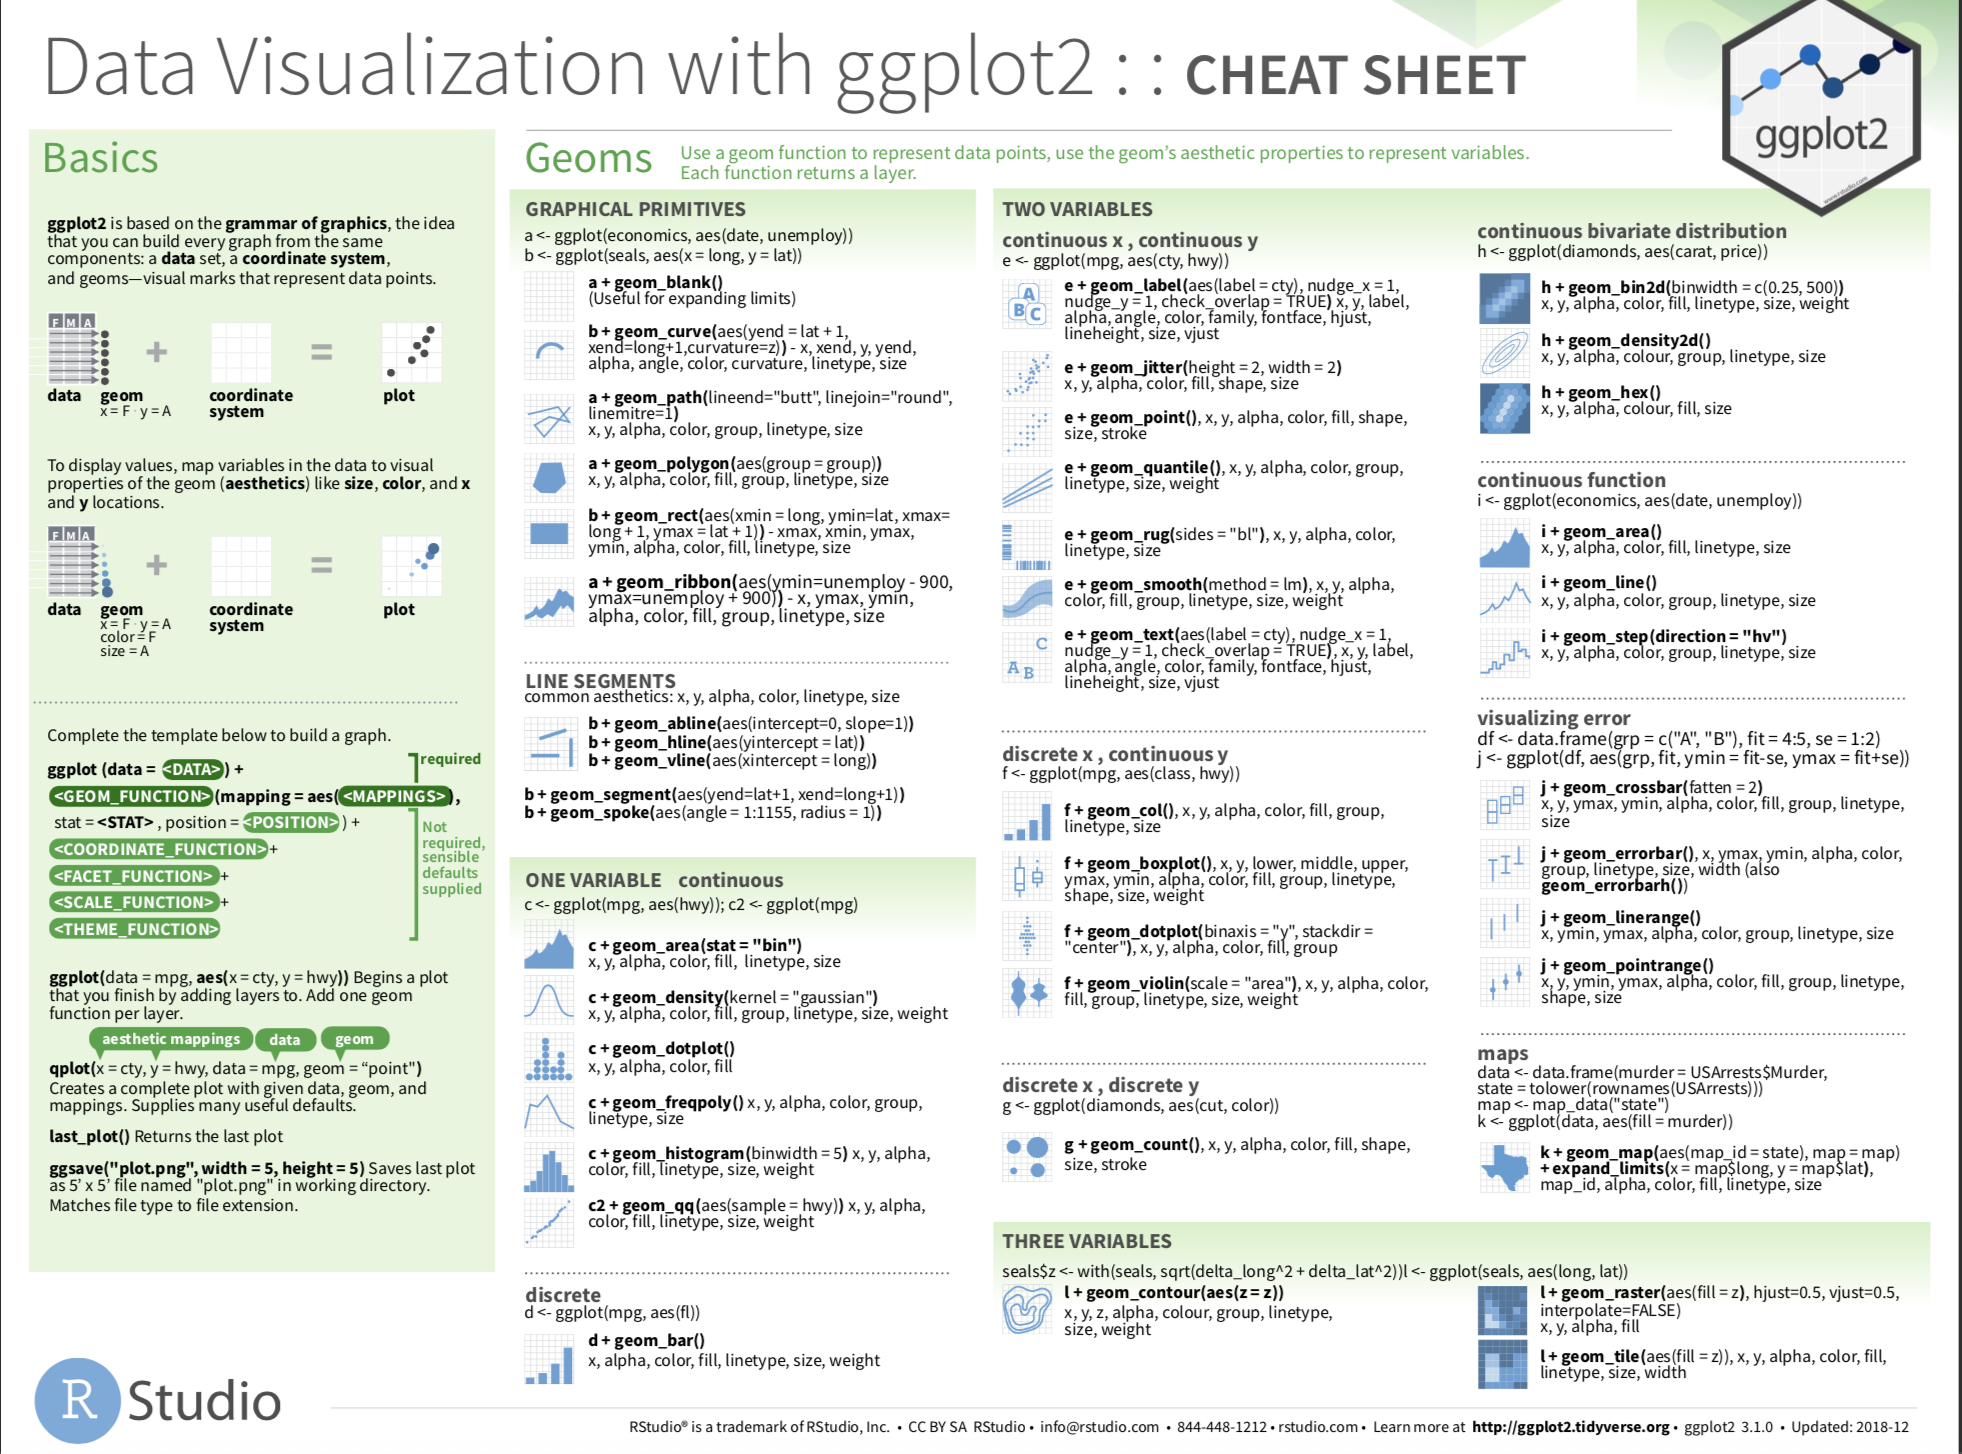
\includegraphics[width=1\textwidth]{figures/data_visualization.png}
    \caption{Official RStudio Cheat Sheet for Data Visualization with 
    ggplot2, "https://www.rstudio.com/resources/cheatsheets/#ggplot2"}
    \label{fig:example_figure}
  \end{center}
\end{figure}


\end{document}

%%% Local Variables:
%%% mode: latex
%%% TeX-master: t
%%% End:
